\begin{tframe}{Literature of Graph Neural Networks}
    GNNs are deep learning based methods that operate on graph domain.
    \vspace{0.2cm}

    \textbf{Applications}: Recommender systems, BioInformatics, Computer Vision\ldots
    \vspace{0.2cm}

    \textbf{Tasks:} Node-Level, Edge-Level, Graph-Level.
    \vspace{0.2cm}

    \begin{minipage}[t]{.5\linewidth}
        \textbf{Benefits of GNNs:}
        \begin{adv}
            \item Modeling relational data;
            \item Generalization to\\ arbitrary graphs;
            \item Capturing complex\\ relationships;
            \item Representation learning.
        \end{adv}
    \end{minipage}%
    \hfill%
    \begin{minipage}[t]{.5\linewidth}
        \textbf{Challenges of GNNs:}
        \begin{disadv}
            \item Scalability;
            \item Data quality and noise;
            \item Model interpretability;
            \item Over-smoothing;
            \item Graph isomorphism problem.
        \end{disadv}
    \end{minipage}
\end{tframe}
%
% \begin{tframe}{Application of KGs}
%     \begin{figure}[htbp]
%         \centering
%      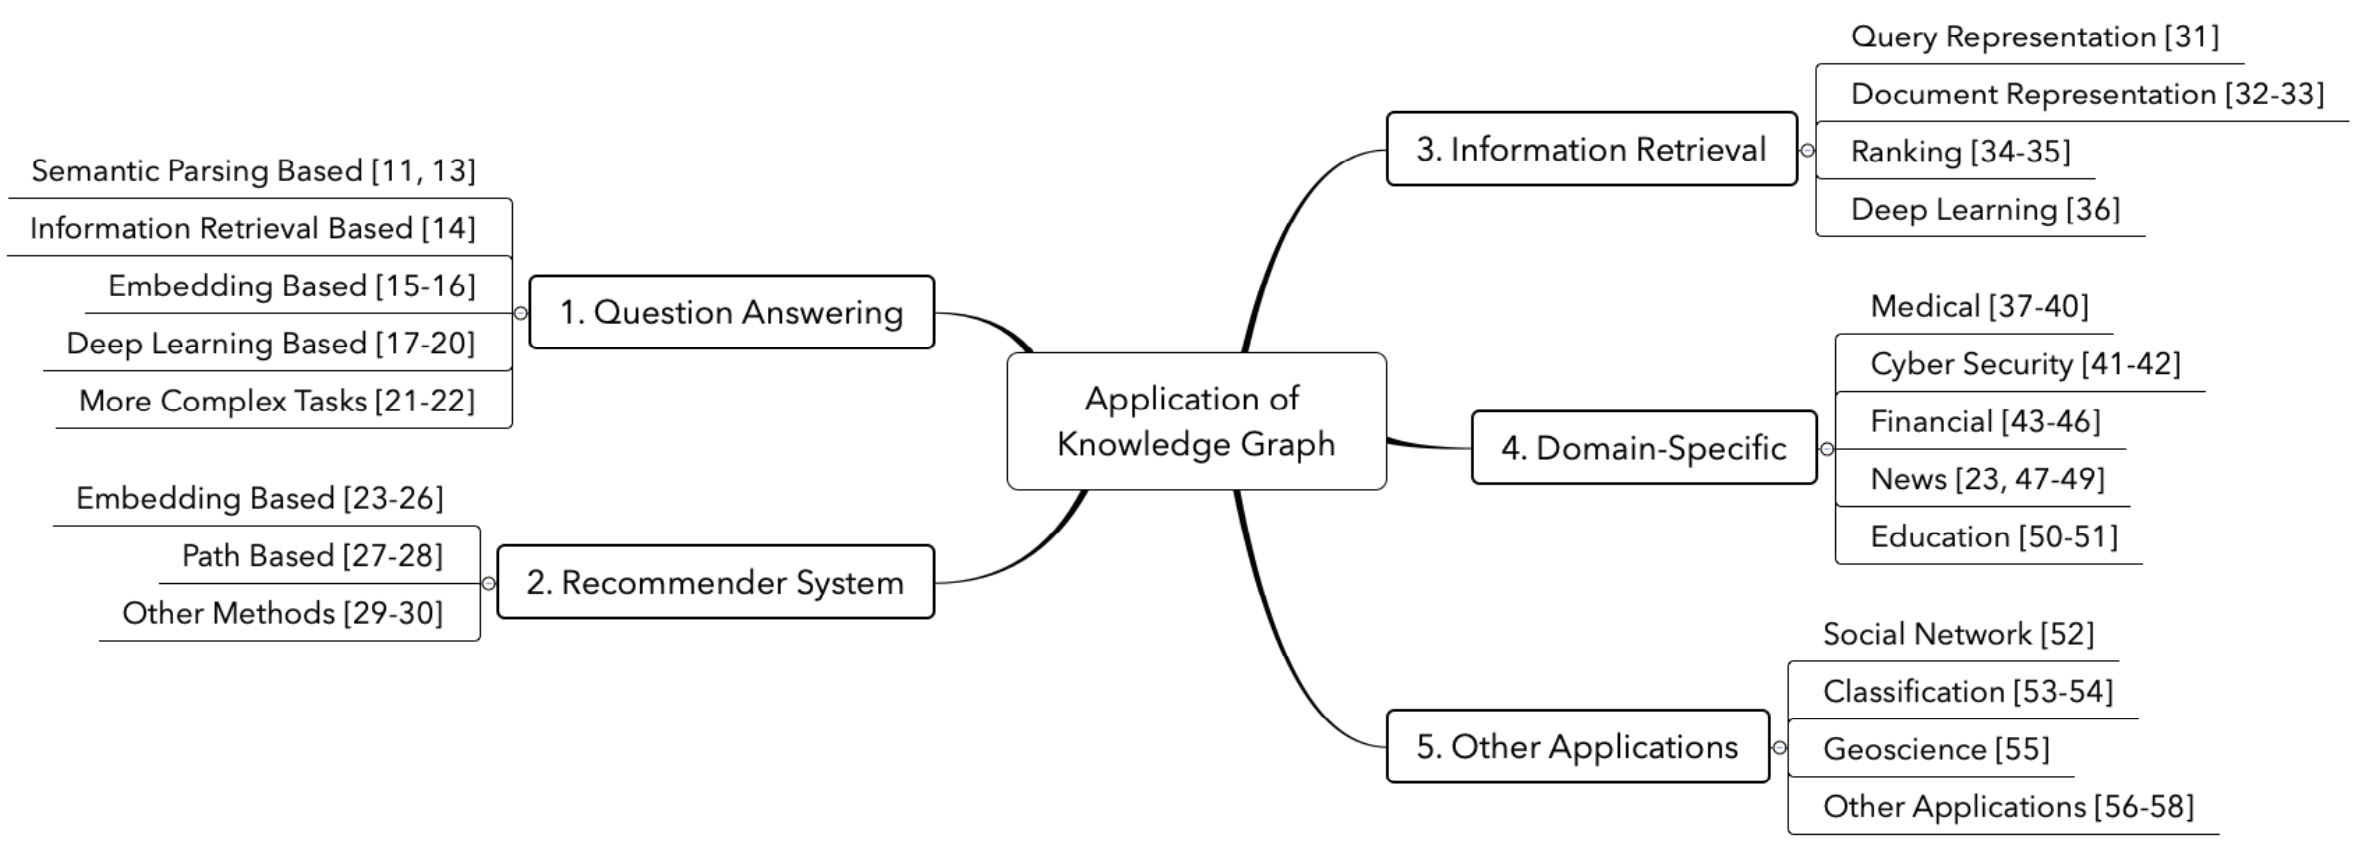
\includegraphics[width=0.9\textwidth]{../img/literature-review/application-field-kg.png}
%      \caption{Application fields of KGs (\cite{Zou2020})}
%     \end{figure}
% \end{tframe}
% \begin{tframe}{Literature of Graph Neural Networks}
% Graph Neural Networks (GNNs) are deep learning based methods that operate on graph domain (non-Euclidean space) (\cite{Wu2021}).
% \newline
% \\ GNNs were introduced when Convolutional Neural Networks (CNNs) failed to achieve optimal results due to the arbitrary size of the graph and complex structure. 
% \newline
% \\ GNN aims to map the node features to node embeddings such that 2 embeddings are ''similar`` if the 2 nodes are ''similar`` in the graph.
% \end{tframe}
% %
% \begin{tframe}{GNN Tasks}
%     \begin{itemize}
%         \item \textbf{Node-Level}: node classification, node regression, node clustering, etc;
%         \item \textbf{Edge-Level}: edge classification and link prediction;
%         \item \textbf{Graph-Level}: graph classification, graph regression, and graph matching.
%     \end{itemize}
% \end{tframe}
% %
% \begin{tframe}{How GNN works}
%     \begin{enumerate}
%         \item \textbf{Message Passing}: is the process of taking node features of the neighbours, transforming them, and ''passing`` them to the source node. This process is repeated, in parallel, for all nodes in the graph. In that way, all neighbourhoods are examined by the end of this step.
%         \item \textbf{Aggregation}: is the process to ''combine`` the transformed messages and the source node together;
%         \item \textbf{Update}: using these aggregated messages, the GNN layer now has to update the source node $\mathnormal{i}$'s features. At the end of this update step, the node should not only know about itself but its neighbours as well. This is ensured by taking the node $\mathnormal{i}$'s feature vector and combining it with the aggregated messages.
%     \end{enumerate}
% \end{tframe}
% %
% \begin{tframe}{The Message Passing Neural Network (MPNN)}
% The MPNN is the most general GNN model:
% \begin{align*}
%     x_i' = \psi(x_i,~\sigma_{j \in N(i)}~ \phi(x_{i},e_{ij},x_j))
% \end{align*}
% where:
% \begin{itemize}
%     \item $\phi$ is a differentiable \textbf{message} funtion;
%     \item $\sigma$ is a permutation-invariant aggregation function (sum, average, etc.)
%     \item $\psi$ is a differentiable \textbf{update} function;
% \end{itemize}
% \end{tframe}